\section{Real-time analysis in physics results}
\label{sec:RTA_physics}
%Caterina having a first go, but students will edit further during circulation period

In this section, we briefly outline and give references for some of the physics analyses that have been performed by ATLAS, CMS and LHCb using real-time analysis (RTA) in Run~1 and Run~2. The success of such analyses has further motivated the development and adoption of RTA techniques in Run~3 trigger systems. %, as summarised in Table~\ref{trigger-table}.

% commenting out this table since it is a repetition of previous sections and it is unclear how it belongs to the physics section
\iffalse

\begin{table}[!ht]
    \centering
    \begin{tabular}{c|p{0.75\linewidth}}
        \thickhline
        \small{\textbf{Experiment}} & \textbf{Summary} \\
        \hline\hline
        \multirow{3}{*}{\small{ALICE}}
            & \small{The ALICE trigger system provides timing to synchronise data from continuous and discrete subdetector readout systems. A software trigger then performs the reconstruction of events, reduction of data volume and calibration of subdetectors (e.g., TPC). The upgrade of many subdetectors to read out data continuously provides a significant increase in the number of collisions which can be collected (i.e., those previously occurring during subdetector dead time).} \\
        \hline
        \multirow{3}{*}{\small{ATLAS}}
            & \small{ATLAS uses a hardware-based L1 trigger to reduce the overall event rate from $40$ MHz to $100$ kHz, using granular information from the calorimeters and the muon systems. A software-based computing farm, the HLT, reduces the L1 output rate down to $\sim$ 1.2 kHz. The second software step utilises full detector reconstruction together with more detailed algorithms for the final selection.} \\ \hline
        \multirow{3}{*}{\small{CMS}}
            & CMS employs a two-level trigger system similar to that of ATLAS. L1 decisions are made on granular information from the calorimeters and muon system. Afterwards, a HLT decision is made using data from all sub-detectors and algorithms including Particle Flow.
            % with relaxed latency requirements. The CMS HLT  farm also comprises of GPUs. 
            \\ \hline
        \multirow{3}{*}{\small{LHCb}}
            & \small{The removal of the L0 trigger requires that HLT1 reduce the event rate by a factor of 30, achieved by the use of GPUs en masse. HLT2 performs offline-quality reconstruction and real-time calibration, with events then saved in the reduced-persistency Turbo format on which analysis can then be performed. Many analyses should receive an improved statistical sensitivity through higher trigger yields and systematic sensitivity by avoiding L0-related systematic effects.} \\
        \thickhline
    \end{tabular}
    \caption{Summary of LHC trigger systems providing input to the real-time analysis data streams.}
    \label{trigger-table}
\end{table}

\fi

% Further comment on Run 3?

%\textbf{Note: this section has not yet been reviewed by CMS SMARTHEP participants, please point out any inaccuracies during the comments period.}
%\subsection{CMS}

The data scouting stream in CMS has been in place since the LHC Run~1, and its first use in searches for dijet resonances is described in Ref.~\cite{CMS:dijet-7tev-resonances} and a review of all CMS scouting searches can be found in Ref.~\cite{CMS:2024zhe}. The RTA approach allows the reach of this search to be extended to resonances with masses as low as \SI{500}{\giga\electronvolt} improving on the standard data-taking analysis that would only be sensitive to resonances with masses of 1 TeV and above\footnote{Other techniques also exist beyond RTA to reach lower resonance masses, e.g., by triggering on initial state radiation or considering boosted jets that contain the resonance products.}. The same search has also been performed with the 8 and 13 TeV centre-of-mass LHC datasets in Run~1 and Run~2, and described in Refs.~\cite{CMS:2016ltu, CMS:2016gsl}, extending the reach to 500 GeV resonances. ATLAS also searched for dijet resonances using the TLA technique, with sensitivity for resonances with masses as low as 450 GeV, as described in Ref.~\cite{ATLAS:2018qto} and shown in Figure~\ref{fig:trigger-level-efficiencies}.

\begin{figure}[!ht]
    \centering
    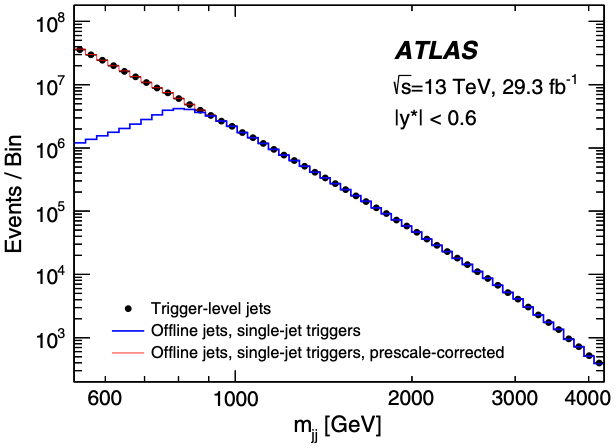
\includegraphics[width=0.55\linewidth]{images/ATLAS-TLA.png}
    \caption{Comparison of offline and trigger-level jet objects in ATLAS dijet spectra from Ref.~\cite{ATLAS:2018qto}. Trigger-level jets allow recording low $m_{jj}$ events at the full rate by greatly reducing the throughput.}
    \label{fig:trigger-level-efficiencies}
\end{figure}

%CD: missing dijet+ISR? 

Searches for multijet resonances (new particles decaying in paired dijet and three jets each) also employ, for example in Ref.~\cite{CMS:scouting-search-multijet}. RTA extends the reach of previous searches to the low mass region from 200 GeV down to 70 GeV for RPV squarks and gluinos. 

Long-lived particles (LLPs) predicted by beyond-SM models decay far from the point of collision, a signature distinct from the promptly decaying particles of the majority of LHC searches. LLPs are often rejected by standard reconstruction algorithms due to their unusual characteristics (e.g., display decay vertices)~\cite{llps}. As such, LLPs require dedicated selection techniques and searches, for example, in CMS real-time searches for dark photons and LLPs decaying into muons using Run~2 data.  Ref.~\cite{CMS:2019buh} describes a search for dark photons decaying into dimuons that uses RTA in the 11.5-45 GeV mass range. In Ref.~\cite{CMS:2021sch}, RTA enables access to the new phase space of low dimuon masses and non-zero displacement that would otherwise not be covered by standard searches.

%\subsection{ATLAS}

%\subsection{LHCb}

In LHCb, real-time analysis was motivated~\cite{Gligorov:2018fuk} by the size of the LHC production cross-section of hadrons containing a charm 
quark. Because this cross-section is so large, it is not possible to record all signal decays of charmed hadrons to permanent storage while keeping the full detector information for each event. Therefore, these decays must be fully reconstructed and selected in real-time, requiring accurate and up-to-date detector alignment and calibration in the real-time processing to keep systematic uncertainties under control. This is particularly crucial since LHCb has a unique ability to probe CP violation in charm hadrons to the $10^{-5}$ level or better, requiring a corresponding control of systematics. For this reason, LHCb implemented the full offline-quality reconstruction, alignment, and calibration~\cite{Dujany:2015lxd, Aaij:2016rxn, Borghi:2017hfp, LHCb:2018zdd, Aaij:2019uij} of the detector within its real-time processing (specifically the software trigger) during Run~2, and adopted real-time analysis as the baseline model~\cite{LHCbCollaboration:2319756} for the majority of the collaboration's physics programme from Run~3 onwards. In Run~2, almost all analyses of charm hadrons, as well as certain searches for BSM states (most notably dark photons), were carried out using real-time analysis.